\chapter{Diseño de los SheetChat}

El diseño de la solución que se ha adoptado para la generación de chatbots o agentes conversacionales utilizando hojas de cálculo se divide en dos partes claramente diferenciadas. Esto es debido al objetivo que se ha presentado en los anteriores apartados, que es generar un chatbot para la consulta de datos extraidos en hojas de cálculo. Tal y como se puede observar en la Figura \ref{fig:featureModel}, por un lado hay que definir el origen de datos, los Sheet u hojas de cálculo. Por otro lado el cómo se consulta los datos, el chat o la conversación que se define para obtener los resultados.

\begin{figure}[htb]
	\centering
	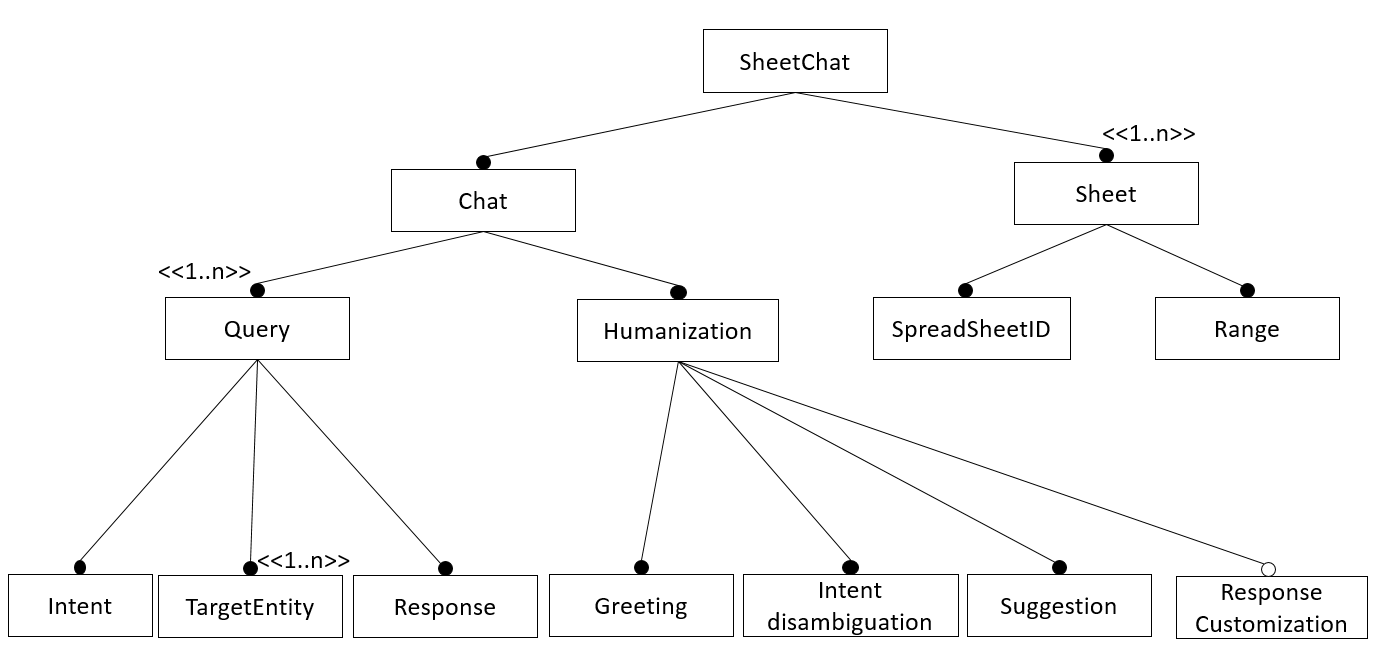
\includegraphics[width=0.8\textwidth]{./figs/FeatureModel.png}
	\caption{Modelo de características de SheetChat.} \label{fig:featureModel}
\end{figure}


En el Apartado \ref{sec:Sheet} se hablará sobre cómo se manejan las hojas de cálculo para su posterior consulta mediante un chatbot. En el Apartado \ref{sec:Chat} se describirá cómo se define un chatbot, el tipo de consultas y el procedimiento para hacerlas. Asimismo se mostrará el cómo se realiza la humanización de un chatbot, que permite mejorar la experiencia de usuario a la hora de conversar.

\section{Sheet}
\label{sec:Sheet}

Las hojas de cálculo son unas herramientas muy potentes que permiten además de generar gráficas o trabajar con complejas funciones matemáticas, el almacenar datos en forma matricial (filas y columnas). Las hojas de cálculo están orientadas al análisis de datos y las bases de datos al almacenamiento de las mismas \cite{Philips2014}, sin embargo, ambas almacenan datos basados en columnas y filas (o tuplas).

En el enfoque de nuestro trabajo, cada hoja de cálculo representa un conjunto de datos en forma de tabla. Al igual que sucede con los ficheros CSV, la primera fila es la cabecera de la tabla, donde se especifica cual es el nombre de cada columna. Las posteriores filas se traducen en tuplas que serán los datos a consultar.

A la hora de definir un chatbot se pueden definir más de un origen de datos. En la tecnología utilizada hay que mencionar que se definen hojas de cálculo en Google SpreadSheet\footnote{Sitio web de Google SpreadSheets: \url{https://www.google.com/sheets/about/}}. La principal ventaja que ofrece esta tecnología es que los datos residen en la nube, lo que permite ser accedidos desde cualquier plataforma y en cualquier momento y siempre se dispondrá de la versión más actualizada de los datos a consultar.

%TODO Explicar los dos campos para identificar el spreadsheet

Los datos que el usuario requiera consultar no serán datos en bruto, si no que el DSL desarrollado permitirá consultas con cierto nivel de riqueza. Para ello se ofrecen funciones matemáticas a la hora de mostrar el resultado o funciones de filtrado. Estas consultas se definen en el sistema de conversación de SheetChat en el Apartado \ref{sec:Consultas}.

\section{Chat}
\label{sec:Chat}

Tras definir el origen de los datos con el que trabajará el chatbot, se ha de definir la interfaz de consultas que tendrá el usuario al realizar las consultas a su hoja de cálculo. Antes de hablar del acceso a los datos, es importante destacar 

%TODO Intents y entities

\subsection{Consultas}
\label{sec:Consultas}

%TODO SQL engine

%TODO relación input-output column

%TODO entities en las que buscar

%TODO funcionalidades de output columns


\subsection{Humanizacion}
\label{sec:Humanization}

%TODO Greeting

%TODO Mensajes customizados

%TODO Mensajes de resultado no encontrado

%TODO Suggestions

